% !TEX root = Master.tex

The methodology is validated by comparing the predicted mean diameter to the mean diameter from the inventory data on compartment level. Figure \ref{fig:radius} depicts the results, whereby the predicted mean radius is obtained by sampling 1000
diameters from the corrected density distribution of the appropriate compartment. Only compartments with 40 or more inventory data points are considered. Table \ref{summary statistics} depicts the summary
statistics of the differences between sampled and observed values.

\begin{figure}[H]
\centering
  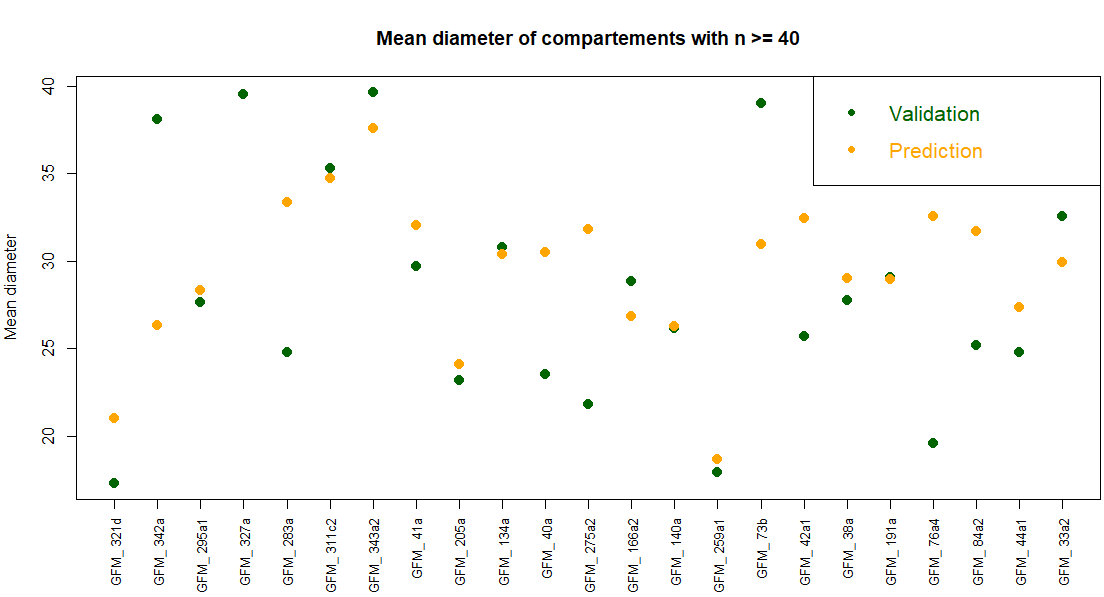
\includegraphics[scale = 0.4]{radius.png}
  \caption{Sampled mean diameter vs observed mean diameter for compartments with sufficient samples.}
  \label{fig:radius}
\end{figure}

\begin{table}[H]
\setlength\arrayrulewidth{1pt}
\centering
\begin{adjustbox}{max width=\textwidth}

\begin{tabular}{|c|c|c|}
\hline 
\rowcolor{Gray}
\textbf{Median} & \textbf{Mean} & \textbf{RSE} \\ 
\hline 
-2.8218 & -2.4574 & 5.487 \\ 
\hline 
\end{tabular} 

\end{adjustbox}

\caption{Summary Statistics of the observed diameter per compartment subtracted the mean sampled diameter}
\label{summary statistics}
\end{table}

The mean diameter is overestimated in the median and mean by 2.82cm and 2.46cm respectively. The residual standard error is 5.487cm.